% 유형 088 155-21(본책 155쪽) — 원을 A, B, C, D(위쪽)·E(아래쪽 큰 영역) 다섯 영역으로 나눈 색칠 영역도. 스캔 그림을 TikZ 로 다시 그림.
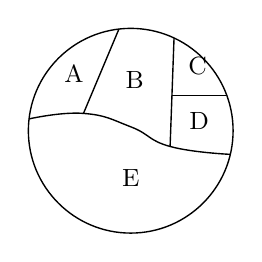
\begin{tikzpicture}[line width=0.5pt, font=\small]
  \draw (0,0) circle (1.3);
  \draw plot[smooth, tension=0.8] coordinates {(-1.291,0.15) (-0.6,0.22) (0,0.05) (0.5,-0.2) (1.264,-0.3)};
  \draw (-0.15,1.291) -- (-0.6,0.22);
  \draw (0.55,1.178) -- (0.5,-0.2);
  \draw (0.524,0.45) -- (1.22,0.45);
  \node at (-0.72,0.72) {$\mathrm{A}$};
  \node at (0.05,0.65) {$\mathrm{B}$};
  \node at (0.85,0.82) {$\mathrm{C}$};
  \node at (0.87,0.12) {$\mathrm{D}$};
  \node at (0,-0.6) {$\mathrm{E}$};
\end{tikzpicture}
